%Removing overlays from a beamer presentation is easily done within the preamble,
%by adding the handout option
%\documentclass[handout,xcolor=pdftex,dvipsnames,table,notheorems]{beamer} 
%\usepackage{pgfpages}
%\pgfpagesuselayout{4 on 1}[a4paper,border shrink=5mm,landscape]

%latex editor online

\documentclass[notheorems,hyperref={bookmarks=true}]{beamer}
\usepackage[framesassubsections]{beamerprosper}
\hypersetup{pdfpagemode=FullScreen}
\usepackage[utf8]{vietnam}
%\usepackage[tcvn]{vietnam}
\usepackage[english]{babel}
\usepackage{ulem} %for underlying+
\usepackage{pifont} %for creating dingautolist
\usepackage[mathscr]{eucal}
\usepackage{amsfonts,amsmath, amsthm, amssymb,amsxtra,latexsym,amscd,graphics,graphpap}
\usepackage{indentfirst}
\usepackage{rotating}
\usepackage{graphicx}
\usepackage{amsbsy}
\usepackage{epsfig}
\usepackage{natbib}
%\usepackage{pst-plot}
%\usepackage{msc}
%\usepackage{musixtex}
\usepackage{pdfpages}
\usepackage{multicol}
\usepackage{hyperref}
\usepackage{subfigure}
\usepackage{multimedia}
\usepackage{boxedminipage}
\usepackage{tikz}
\usepackage{nicefrac}
\usepackage{tabu}
\setbeamertemplate{theorems}[numbered] % Đánh số định lý.
%\usetheme{Warsaw}
%\usetheme{Berlin}
%\usetheme{Madrid} 
%\usetheme{boadilla} 
%\usetheme{CambridgeUS} 
%\usetheme{Goettingen}
%\usetheme{Boadilla} % puts title, section, etc on top
%\usetheme{PaloAlto} % top and left bar.  left bar has outline
%\usetheme{Berkeley} % similar to Palo Alto
%\usetheme{Hannover}  % left bar with outline
%\usetheme{AnnArbor}
%\usetheme{Pittsburgh}
%\usetheme{Antibes}
%\usetheme{JuanLesPins}
%\usetheme{Montpellier}
%\usetheme{Szeged}
\usetheme{Copenhagen}
\usecolortheme{rose} 
\usefonttheme[onlylarge]{structurebold}
\usefonttheme{professionalfonts}
%\useoutertheme{smoothbars}

\setbeamercolor{title}{fg=red!80!blue,bg=blue!20!white}
\setbeamertemplate{section in head/foot shaded}[default][20]
\setbeamertemplate{subsection in head/foot shaded}[default][20]
\setbeamertemplate{navigation symbols}{}
\setbeamertemplate{blocks}[rounded][shadow=true]
\setbeamerfont{small}{size=\small}
\setbeamerfont{footnote}{size=\footnotesize}
\setbeamerfont{script}{size=\scriptsize}
\setbeamerfont{tiny}{size=\tiny}

\providecommand{\R}{\mathbb{R}}
\providecommand{\Mat}{\textsc{MatLab }}
%\providecommand{\lr}[1]{\left( #1 \right)} 
%\providecommand{\Lr}[1]{\left[ #1 \right]}
%\providecommand{\LR}[1]{\left\{ #1 \right\}} 
%\providecommand{\abs}[1]{\left\vert #1 \right\vert} 
%\providecommand{\norm}[1]{\left\Vert #1 \right\Vert} 
\providecommand{\ov}[1]{\overline {#1}} 
\providecommand{\e}{\varepsilon} 
\DeclareMathSymbol{\INT}{\mathop}{largesymbols}{"5A} 
\renewcommand{\int}{\INT} 
\renewcommand{\iint}{\mathop{\int\!\!\!\!\!\int}}
\renewcommand{\iiint}{\mathop{\int\!\!\!\!\!\int\!\!\!\!\!\int}}
\DeclareMathOperator{\sinc}{sinc}

\theoremstyle{plain}
%\theorembodyfont{\slshape}
\newtheorem{definition}{Định nghĩa}[section]
\newtheorem{proposition}{Mệnh đề}[section]
\newtheorem{theorem}{Định lý}[section]
\newtheorem{lemma}{Bổ đề}[section]
\newtheorem{corollary}{Hệ quả}[section]
\newtheorem{conjecture}{Dự đoán}[section]
\newtheorem{remark}{Chú ý}[section]
\newtheorem{example}{Ví dụ}
\newtheorem{problem}{Bài toán}[section]
\newtheorem{exercise}{Bài tập}

\renewcommand{\thedefinition}{\arabic{section}.\arabic{definition}}
\renewcommand{\thelemma}{\arabic{section}.\arabic{lemma}}
\renewcommand{\thetable}{\Roman{table}}
\renewcommand{\thetheorem}{\arabic{section}.\arabic{theorem}}
\renewcommand{\thecorollary}{\arabic{section}.\arabic{corollary}}
\renewcommand{\theequation}{5.\arabic{section}.\arabic{equation}} 
\renewcommand{\thefootnote}{(\arabic{footnote})}
\renewcommand{\theexample}{\arabic{example}}
\renewcommand{\theproblem}{\arabic{section}.\arabic{problem}}
\renewcommand{\theexercise}{\arabic{exercise}}
\mode<presentation>
\setbeamertemplate{navigation symbols}{} 
%\logo{\includegraphics[height=1cm]{logo.pdf}}
%\logo{%
%    \includegraphics[width=1cm,height=1cm,keepaspectratio]{logo.pdf}~%
%    \includegraphics[width=1cm,height=1cm,keepaspectratio]{logo.pdf}~%    
%}
%\pgfdeclareimage[height=1cm]{fami-logo}{Logo-khoa-chup}
%\pgfdeclareimage[height=1.5cm]{hust-logo}{logo}
%\logo{\pgfuseimage{fami-logo}}
%\setbeamertemplate{footline}{\raisebox{-2.2ex}{\pgfuseimage{hust-logo}}}

\title[{\makebox[.45\paperwidth]{Xemina Tin}}]{Mô hình hồi quy Logistic } 
\author[NHÓM 3 ]{NHÓM 3 \\
Lai Đức Thắng - 20163830\\
GVHD : TS. TRẦN MẠNH TUẤN}
\institution[SAMI-HUST]{Viện Toán ứng dụng và Tin học, ĐHBK Hà Nội}
\date{Hà Nội, tháng 07 năm 2020}

\renewcommand{\sfdefault}{cmss}
\renewcommand{\rmdefault}{cmr}
\renewcommand{\ttdefault}{cmtt}


\begin{document}
\begin{footnotesize}
\begin{frame}
	\frametitle{}
	\maketitle
%	\begin{block}
%	\titlepage
%	\end{block}
\end{frame}

\AtBeginSection[] % Do nothing for \section*
{
	\begin{frame}<beamer>
		\frametitle{Nội dung}
		\tableofcontents[currentsection, currentsubsection]
	\end{frame}
}
%%%%%%%%%%%%%%%%%%%%%%%%


\begin{frame}
\frametitle{Tổng quan } % Table of contents slide, comment this block out to remove it
\tableofcontents % Throughout your presentation, if you choose to use \section{} and \subsection{} commands, these will automatically be printed on this slide as an overview of your presentation
\end{frame}

%=====================================
\subsection{Vĩnh thức}
\begin{frame}{Vĩnh thức}
Giả sử $M= (m_{ij})$ là ma trận số thức $n \times n$. Khi đó vĩnh thức (Permanents) của ma trận $M$ (kí hiệu là $per$):
\begin{equation*}
per M = \displaystyle \sum_{\sigma \in S_{n}}m_{1\sigma(1)}m_{2\sigma(2)}...m_{n\sigma(n)}
\end{equation*}
trong đó $S_{n}$ là tập tất cả các hoán vị của $\{1,2,...,n\}$.
\end{frame}

\subsection{Hình vuông Latin}
\begin{frame}{Khái niệm}
\begin{table}[ht]
\centering
\begin{tabular}{|c|c|c|c|}
    \hline
     1&2&3&4  \\ \hline
     2&1&4&3  \\ \hline
     4&3&1&2  \\ \hline
     3&4&2&1  \\
     \hline
\end{tabular}
\caption{Hình vuông Latin bậc 4.}
\end{table}
\end{frame}

\begin{frame}{Bài toán}
Xét bài toán: Xác định số hình vuông latin $L(n)$ bậc $n$. Xét một vài ví dụ nhỏ :\\
$n=1$:
\begin{tabular}{|c|}
    \hline
     1 \\ \hline
    
\end{tabular}: ~~~ $L(1) = 1$
\vspace{20pt}
\\
$n=2$:
\begin{tabular}{|c|c|}
    \hline
     1&2 \\ \hline
     2&1 \\ 
     \hline
\end{tabular} ~~~~~~~~
\begin{tabular}{|c|c|}
    \hline
     2&1 \\ \hline
     1&2 \\ 
     \hline
\end{tabular}: ~~~ $L(2) = 2$
\vspace{20pt}
\\
$n=3$:
\begin{tabular}{|c|c|c|}
	\hline
	1&2&3 \\ \hline
	2&3&1 \\ \hline
	3&1&2 \\
	\hline
\end{tabular}: ~~~ $L(3) = 12$

\begin{equation*}
L(1) = 1, L(2) = 2, L(3) = 12, L(4) = 576, L(5) = 161280
\end{equation*}
\end{frame}

\begin{frame}{Bài toán}
Xét bài toán: Xác định số hình vuông latin $L(n)$ bậc $n$. Xét một vài ví dụ nhỏ :\\
$n=1$:
\begin{tabular}{|c|}
    \hline
     1 \\ \hline
    
\end{tabular}: ~~~ $L(1) = 1$
\vspace{20pt}
\\
$n=2$:
\begin{tabular}{|c|c|}
    \hline
     1&2 \\ \hline
     2&1 \\ 
     \hline
\end{tabular} ~~~~~~~~
\begin{tabular}{|c|c|}
    \hline
     2&1 \\ \hline
     1&2 \\ 
     \hline
\end{tabular}: ~~~ $L(2) = 2$
\vspace{20pt}
\\
$n=3$:
\begin{tabular}{|c|c|c|}
	\hline
	1&2&3 \\ \hline
	2&3&1 \\ \hline
	3&1&2 \\
	\hline
\end{tabular}: ~~~ $L(3) = 12$

\begin{equation*}
L(1) = 1, L(2) = 2, L(3) = 12, L(4) = 576, L(5) = 161280
\end{equation*}

\begin{equation*}
? \leq L(n) \leq ?
\end{equation*}
\end{frame}

\begin{frame}{Mô hình bài toán}
Xét một hình vuông $n \times n$ và điền vào đó các số $1,2,..,n$ sao cho đó là một hình vuông Latin

\begin{flushright}
\begin{tabular}{|c|c|c|c|}
	\hline
	2&4&1&3 \\ \hline
	&&& \\ \hline
	&&& \\ \hline
	&&& \\
	\hline
\end{tabular}
\end{flushright}

\end{frame}

\begin{frame}{Mô hình bài toán}
\begin{flushleft}
Xét một đồ thị hai phía $G_k = (U \cup V,E)$, trong đó $U$ là tập các phần tử $\{1,2,..,n\}$ và $V$ là tập các vị trí của cột, sao cho:
\begin{equation*}
ij \in E :\Leftrightarrow i \textrm{ không xuất hiện trong cột thứ } j \textrm{ của } R.
\end{equation*}
\end{flushleft}

\begin{flushright}
	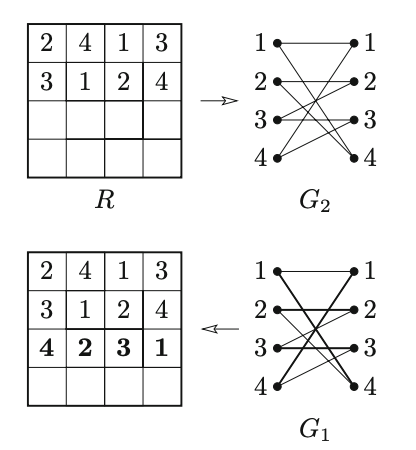
\includegraphics[width=5cm,height=5cm]{ex3}
%	\caption{Đồ thị hai phía với $\mathfrak{S}$ là tập các perfect matching}
\end{flushright}

\end{frame}


\subsection{Phân tích hồi quy}
\begin{frame}{Phân tích hồi quy}
\begin{itemize}
    \item \textbf{Phân tích hồi quy} nghiên cứu sự phụ thuộc của một biến trả lời
(response variable) vào một hoặc nhiều biến dự báo (predictors).
\begin{itemize}
    \item $(x_1, x_2,\dots, x_D)$ : các biến dự báo ( là các thành phần xác định được)
    \item $y$: biến trả lời
\end{itemize}
\item Có 2 dạng phân tích hồi quy:
\begin{itemize}
    \item Hồi quy tuyến tính
    \item Hồi quy phi tuyến
\end{itemize}
\end{itemize}
    
\end{frame}
\begin{frame}{Hồi quy tuyến tính}
Hàm dự báo $h_{\theta}(\textbf{x})$ được xấp xỉ bởi một hàm tuyến tính của \textbf{x}.
\begin{align*}
   h_{\theta}(\textbf{x})=\theta_0 + \theta_1x_1 +\dots +\theta_Dx_D
\end{align*}
Nếu bổ sung thêm đặc trưng cố định $x_0 \equiv 1$  thì ta có thể biểu diễn $h$  dưới
dạng
 \begin{align*}
     h_{\theta}(\textbf{x})= \sum_{j=0}^D \theta_jx_j = \theta^T\textbf{x}.
 \end{align*}  
\end{frame}

\subsection{Giới thiệu}
\begin{frame}
\frametitle{Giới thiệu }
\begin{enumerate}
    \item Mô hình hồi quy logistic được sử dụng rộng rãi trong nhiều bài toán
thống kê và học máy
\item Là một mô hình hồi quy nhằm dự đoán giá trị đầu ra rời rạc (discrete target variable) ứng với một véc tơ đầu vào. Việc này tương đương với chuyện phân loại các đầu vào $x$ vào các nhóm $y$ tương ứng ( Bài toán phân loại)
\item Ví dụ: một bức ảnh có chứa một con mèo hay không. Thì ở đây ta coi đầu vào là các pixel của bức ảnh, đầu ra  y=1 nếu bước ảnh có một con mèo và y=0 nếu bức ảnh không có con mèo nào. 
\item Để đơn giản, nhóm em đã tìm hiểu mô hình và cách giải quyết cho bài toán phân loại nhị phân tức là $y= \{0,1\}.$



\end{enumerate}
\end{frame}

\begin{frame}{Ví dụ thực tế}

Mô hình nghiên cứu mối quan hệ quả bệnh tim và độ tuổi.
Trong bảng số liệu thống kê sau, biến CD = 1 tức là người đó có mắc bệnh tim và CD =0 tức là người đó không mắc bệnh tim. Dựa vào dữ liệu thống kê lớn với đa dạng độ tuổi người ta tìm cách trả lời câu hỏi liệu có mối quan hệ nào giữa độ tuổi và khả năng bị bệnh tim của một người hay không?
\begin{figure}
    \centering
%    \includegraphics[scale = 0.55]{Nga/data2.JPG}
    
\end{figure}
Đây là một phần nhỏ trong dữ liệu thô của 100 người tham gia nghiên cứu.     
\end{frame}

\begin{frame}
    Chúng ta có thể nhóm mỗi người trong ví dụ trên vào các nhóm tuổi và quan sát tỷ lệ phần trăm mắc bệnh tim.
    \begin{figure}
%        \centering    \includegraphics[scale = 0.56]{Nga/data3.JPG}
    \end{figure}
\end{frame}
%=====================================

%%%%%%%%%%%%%%%%%%%%%%%%%%%%%%%
\end{footnotesize}
\end{document}

